
%-------------------------------------------------------------------------------
\chapter{Análise do Problema}
\label{sec:AP}

Neste próximo capítulo aborda-se a análise do problema em questão. Inicia-se com a descrição do domínio do problema, através do glossário de termos usados, do modelo de domínio e do mapa de materialidade da Devscope de acordo com as métricas indicadas pela \gls{SASB} para o setor de \textit{software} e serviços IT. Por fim, serão delineados os requisitos funcionais e não funcionais do sistema.

\section{Contexto}
\label{sec:Context}

A fase de análise é uma das mais importantes no ciclo de vida do desenvolvimento de software, pois é nela que ocorre a recolha dos requisitos, funcionalidades e necessidades do cliente, bem como das especificações do sistema. O objetivo final é definir de forma clara os recursos e funcionalidades que compõem a solução a ser desenvolvida.

Qualquer informação incorreta ou não obtida pode comprometer o desenvolvimento do produto, tanto em termos de qualidade como de cumprimento dos prazos.

A proposta de desenvolvimento de uma plataforma ESG surgiu da necessidade identificada pela Devscope em centralizar e otimizar o controlo de diversas métricas relacionadas com os pilares ambiental, social e de governança (ESG). Esta necessidade prende-se com a crescente importância de monitorizar e reportar práticas sustentáveis, promovendo uma gestão mais transparente, eficiente e alinhada com os objetivos de responsabilidade corporativa da empresa. Ao centralizar estes dados numa única plataforma, a Devscope pretende não só melhorar a sua capacidade de análise e tomada de decisões, como também reforçar o seu compromisso com a sustentabilidade e o impacto positivo na sociedade.

\section{Domínio do problema}
\label{sec:DP} 

A presente secção visa descrever o domínio do problema através de vários artefactos de variadas complexidades, nomeadamente conceitos e diagramas.

A Tabela \ref{tab:glossario_dominio} apresenta os conceitos introduzidos no domínio do problema e que serão usados ao longo do desenvolvimento.

\begin{table}[H]
    \rowcolors{2}{purple!10}{white}
    \renewcommand{\arraystretch}{1.2}
    \setlength{\tabcolsep}{10pt}
    \centering
    \begin{tabular}{>{\bfseries}p{2.5cm} >{\bfseries}p{4cm} p{8cm}}
        \rowcolor{purple!40}
        Conceito (EN) & Conceito (PT) & \textbf{Descrição} \\
        ESG & ESG (Ambiente, Social, Governança) & Conjunto de critérios que avaliam o desempenho ambiental, social e de governança de uma organização, com foco na sustentabilidade e responsabilidade corporativa. \\
        Dashboard & Painel & Resumo gráfico de várias informações importantes, normalmente utilizado para dar uma visão geral de um negócio. \\
        Materiality Map & Mapa de Materialidade & Ferramenta que destaca as métricas ESG mais relevantes para cada setor, segundo as normas da SASB. \\
        Metric & Métrica & Unidade de medida usada para quantificar aspectos específicos do desempenho ESG, como emissões de carbono, diversidade na força de trabalho ou políticas anticorrupção. \\
        PoC & Prova de Conceito & Implementação inicial e simplificada de um sistema ou funcionalidade com o objetivo de validar uma ideia, conceito ou abordagem técnica. \\
        Dataset & Conjunto de Dados & Coleção estruturada de dados ESG, normalmente em formato tabular, que contem informações como categorias, datas e valores associados. \\
        URL & URL (Localizador Uniforme de Recursos) & Endereço que identifica e localiza um recurso na internet, como páginas web, APIs ou arquivos. \\
        API & API (Interface de Programação de Aplicações) & Conjunto de regras que permite a comunicação entre diferentes sistemas ou componentes de \textit{software}. Utilizada para integrar funcionalidades ou aceder a dados. \\
        AWS S3 & AWS S3 (\textit{Amazon Simple Storage Service}) & Serviço de armazenamento em nuvem da \textit{Amazon} utilizado para guardar arquivos como documentos, imagens ou exportações de dados de forma segura e escalável. \\
    \end{tabular}
    \caption{Glossário do domínio do problema}
    \label{tab:glossario_dominio}
\end{table}


A Figura \ref{fig:domain_model} ilustra o modelo de domínio e relaciona os diferentes conceitos da solução.

O \textit{dashboard} apresenta a pontuação ESG consolidada da empresa, oferecendo uma visão geral do seu desempenho em sustentabilidade. Além disso, destaca as métricas mais relevantes, assim como aquelas que apresentaram melhorias ou quedas em relação ao último registro.

Outra seção da plataforma disponibiliza uma visão detalhada de todas as métricas existentes: métricas customizáveis (criadas pelos próprios utilizadores) e métricas orientadas pelos padrões definidos pela \gls{SASB}.

% - Modelo de dominio (diagrama)
\begin{figure}[H]
    \centering
    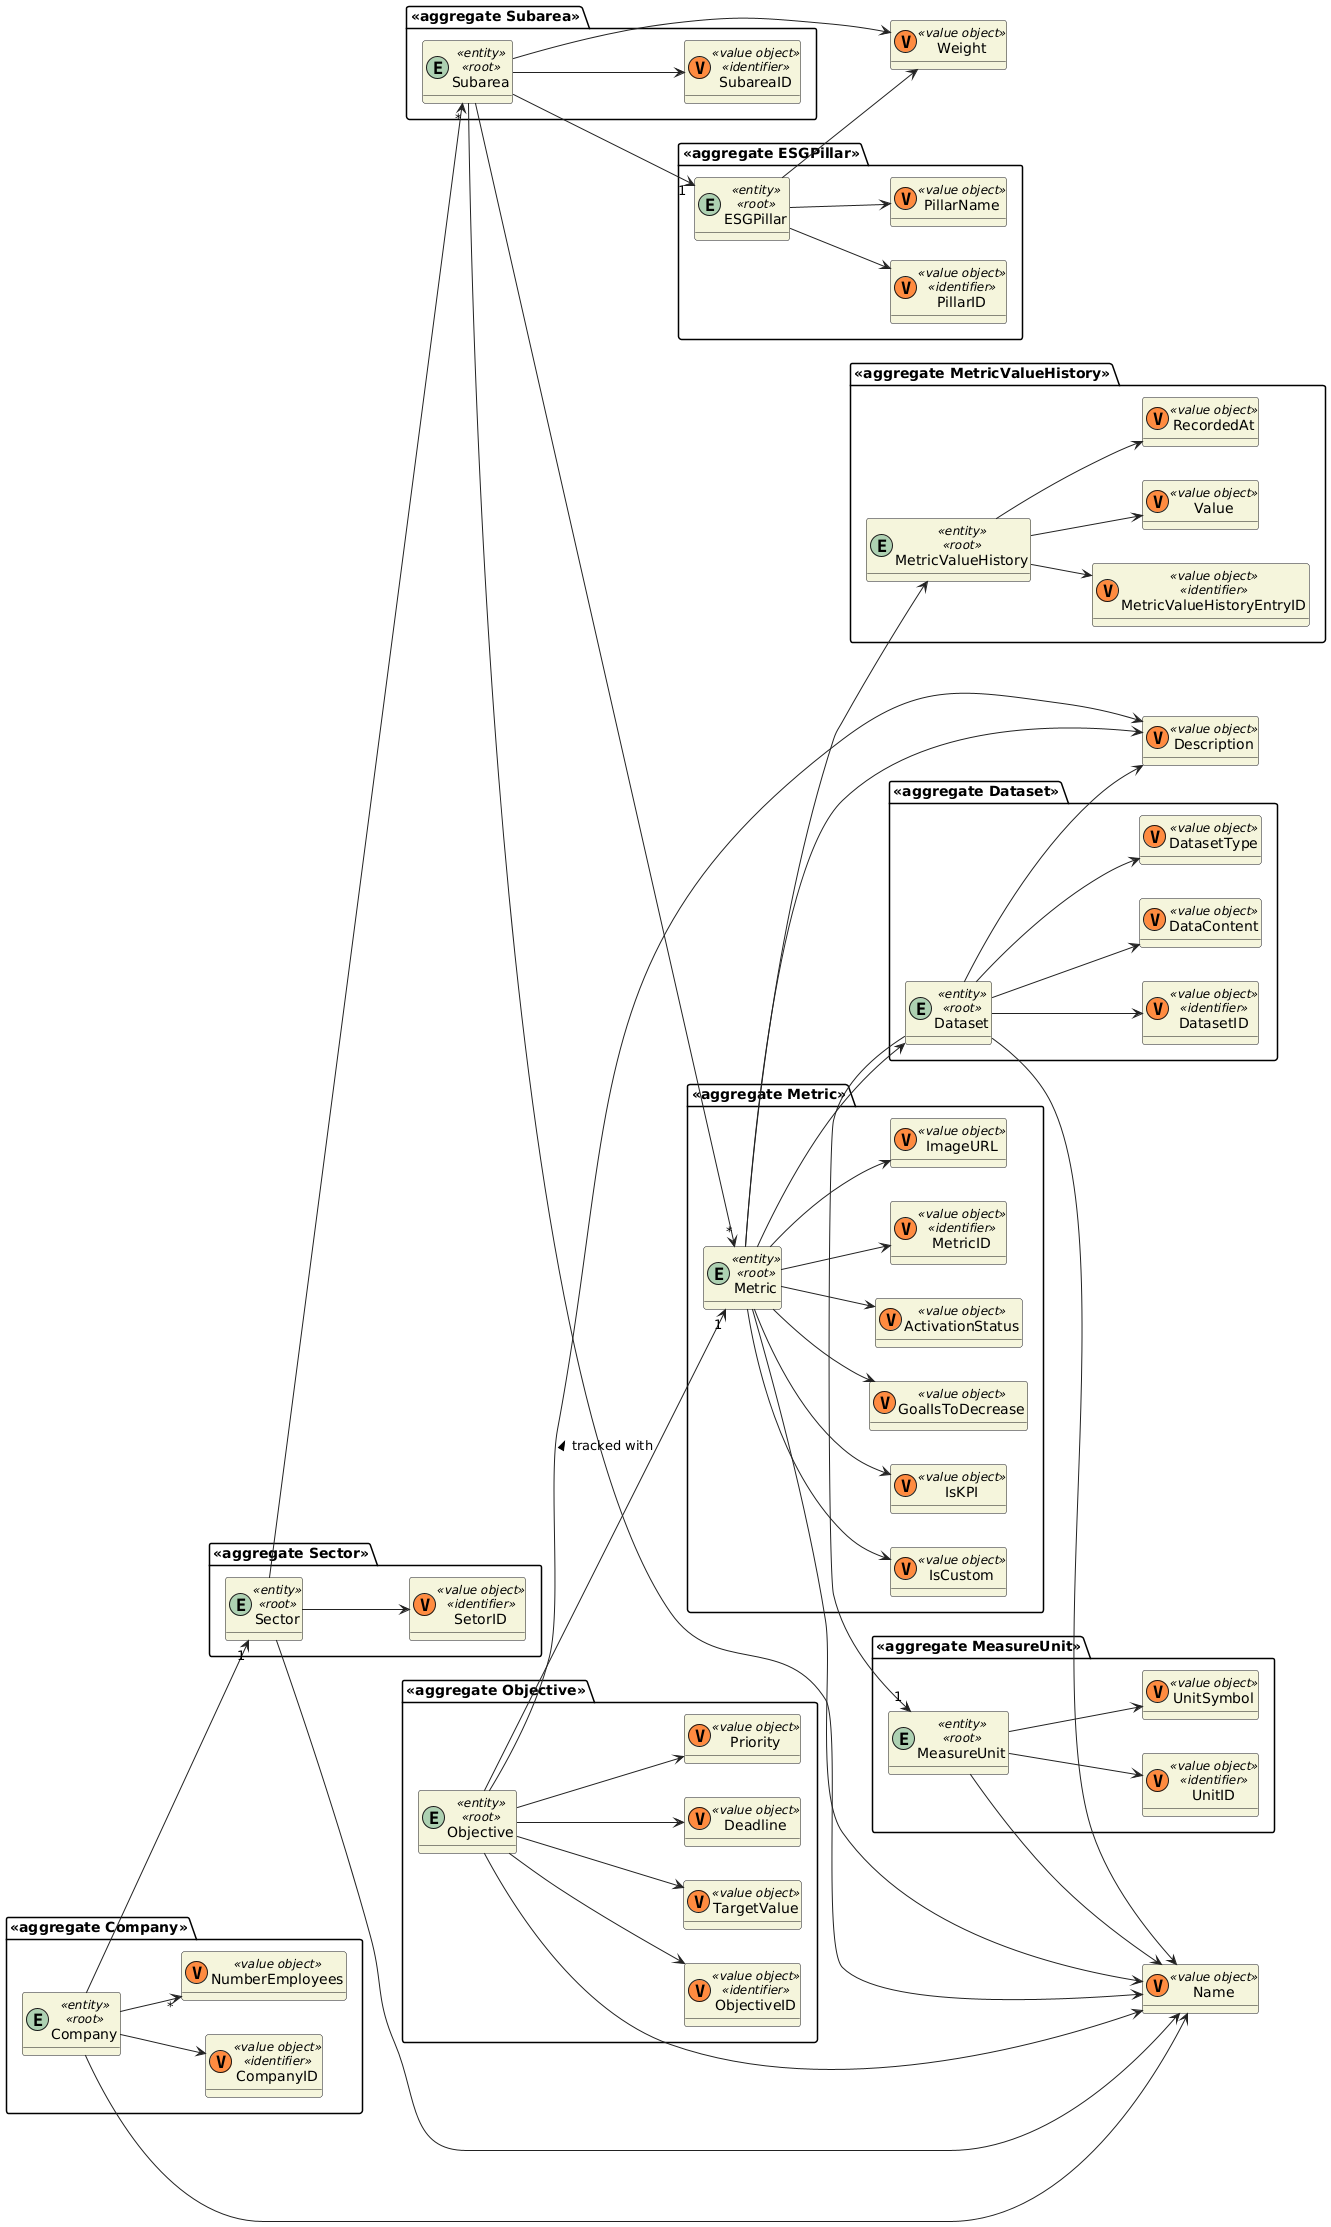
\includegraphics[width=\linewidth,keepaspectratio]{frontmatter/assets/diagrams/Domain Model/Domain_Model2.png}
    \caption{Modelo de Dominio}
    \label{fig:domain_model}
\end{figure}

Cada métrica possui atributos específicos, incluindo o pilar e subárea ESG a que pertence, o seu código identificador, os conjunto de dados que lhe estão associados, a unidade de medida associada aos mesmos e a classificação do seu progresso.

De acordo com a \gls{SASB}, adotado pela Devscope neste projeto, existem normas específicas para cada setor — como é o caso do setor de \textit{Software} e Serviços de TI — que determinam quais as métricas devem ser reportadas (\cite{SASBSector2025}). É com base nestas diretrizes que se constrói o \textbf{Mapa de Materialidade}, como indicado na Figura \ref{fig:materiality_map}.

Este mapa, um dos elementos centrais da plataforma, reflete as métricas ativas não só definidas pela \gls{SASB}, consoante o setor da empresa, bem como as métricas personalizadas. Este mapa organiza as métricas segundo os pilares ESG e respectivas subáreas, e atribui uma cor correspondente ao seu progresso, proporcionando uma visão estruturada das prioridades de sustentabilidade da organização.

% - mapa de materialidade da DevScope (Software e IT sector - SASB)
\begin{figure}[h]
    \centering
    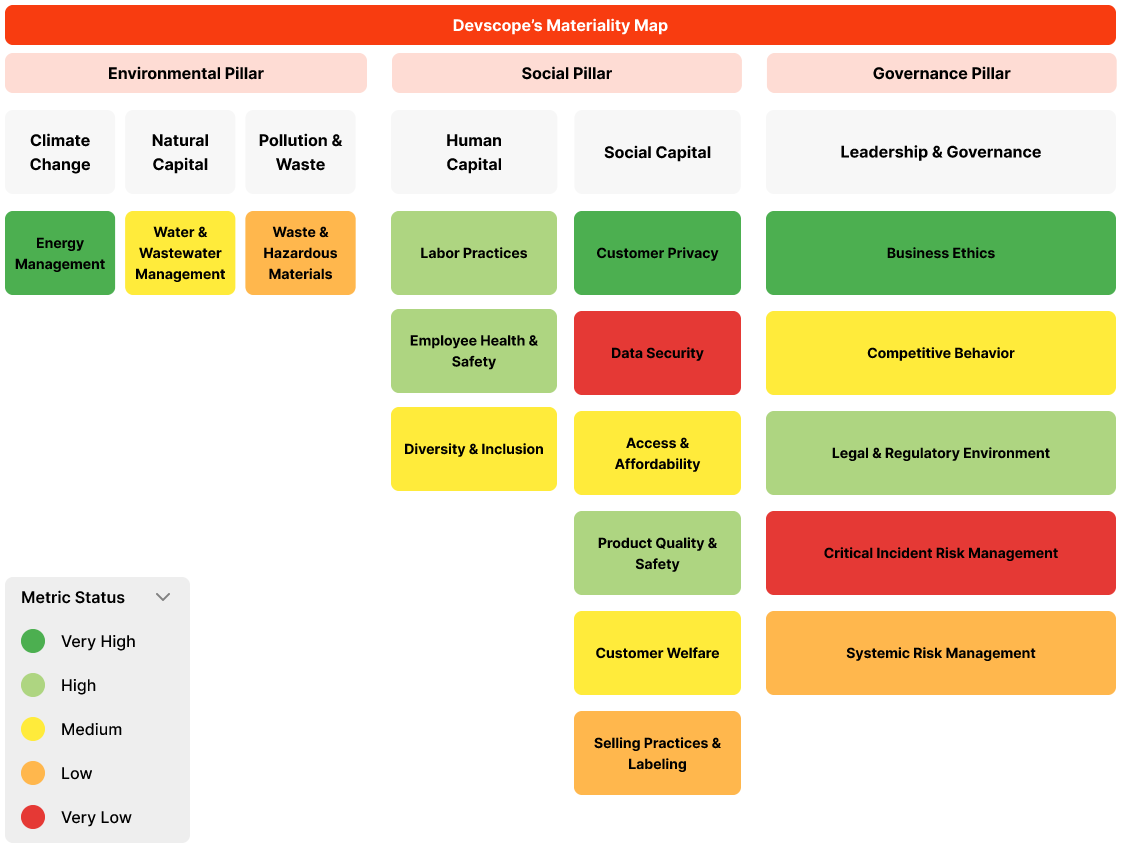
\includegraphics[width=\linewidth]{frontmatter/assets/mapa-materialidade.png}
    \caption{Mapa de Materialidade segundo o setor SASB da Devscope (\textit{Software} e serviços IT)}
    \label{fig:materiality_map}
\end{figure}

Por fim, outra página da plataforma é dedicada à gestão de objetivos, permitindo acompanhar os objetivos definidos, as métricas a eles associadas, o progresso na sua concretização ao saber se se encontram dentro ou fora do plano estabelecido.

\section{Requisitos funcionais e não funcionais}

A seguinte seção compila os requisitos obtidos com o cliente e categoriza-os entre funcionais e não funcionais.

\section{Requisitos Funcionais}

Os requisitos funcionais correspondem a funcionalidades presentes no \textit{software} a ser desenvolvido, normalmente representadas por casos de uso e acompanhados por diagramas. Os requisitos funcionais deste projeto estão organizados na Tabela \ref{tab:use_cases}, onde cada requisitos é considerado um caso de uso e identificado por um código alfa-numérico.

%- Use Cases list
\begin{table}[H]
    \rowcolors{2}{orange!20}{white}
    \renewcommand{\arraystretch}{1.2}
    \setlength{\tabcolsep}{10pt}
    \centering
    \begin{tabular}{>{\bfseries}p{3.5cm} p{4cm} p{7cm}}
        \rowcolor{orange!50}
        Código & \textbf{Descrição Curta} & \textbf{Descrição} \\
        UC-01 & Visualização de KPI's & Como utilizador da plataforma, quero visualizar rapidamente os principais KPIs ambientais, sociais e de governação, para poder avaliar o desempenho da organização. \\
        UC-02 & Filtragem de Métricas & Como utilizador da plataforma, quero poder filtrar os dados por pilar, de modo a facilitar a navegação. \\
        UC-03 & Mapa de Materialidade & Como utilizador da plataforma, quero visualizar a matriz de materialidade dividida por categorias ESG com um sistema de cores intuitivo, para identificar rapidamente os temas mais críticos e, ao clicar em cada indicador, aceder a detalhes explicativos que me ajudem a compreender o seu progresso e evolução. \\
        UC-04 & Pontuação ESG & Como utilizador da plataforma, quero aceder a uma pontuação ESG agregada, para ter uma visão geral do desempenho da empresa em responsabilidade social, ambiental e de governança. \\
        UC-05 & Detalhes de Métricas & Como utilizador da plataforma, quero clicar numa métrica e ver mais detalhes, para compreender a progressão de cada indicador. \\
        UC-06 & Métricas Customizáveis & Como utilizador da plataforma, quero poder criar métricas ESG específicas à realidade da empresa e definir a sua fonte de dados, para garantir que o painel reflete os indicadores mais relevantes para a nossa estratégia. \\
        UC-07 & Importe de Dados & Como utilizador da plataforma, quero poder importar dados para associar às métricas. \\      
    \end{tabular}
    \caption{Lista de Casos de Uso}
    \label{tab:use_cases}
\end{table}

Alguns casos de uso partilham entre si a mesma estrutura de interação representada nos diagramas da vista de processos — detalhada na Subseção \ref{subsec:process_view}. Exemplos disso são os casos de uso \textbf{UC-01, UC-02, UC-03, UC-04} e \textbf{UC-05}, que seguem a sequência ilustrada na Figura \ref{fig:UC12345-lvl1}, variando apenas no conceito de negócio específico que cada um aborda.

\begin{figure}[h]
\centering
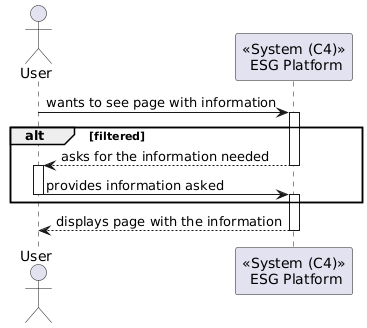
\includegraphics[width=4in]{frontmatter/assets/diagrams/Process Views/UC12345-lvl1.png}
\caption{Vista de processos dos casos de uso de consulta/visualização e filtragem (Nível 1)}
\label{fig:UC12345-lvl1}
\end{figure}


\subsection{UC-01 | Visualização de KPI's}

\textbf{Objetivo:} Permitir ao utilizador consultar rapidamente os principais indicadores-chave de desempenho (KPIs) ESG da organização. \\
\textbf{Ator Principal:} Utilizador da plataforma \\
\textbf{Descrição Geral:} Este caso de uso disponibiliza uma visão geral de métricas dos três pilares (Ambiental, Social e de Governação). A interface mostra indicadores como emissões de CO$_2$, diversidade na força de trabalho, entre outros. \\
\textbf{Fluxo Principal:}
\begin{enumerate}
    \item O utilizador acede ao painel principal da plataforma.
    \item A aplicação apresenta os KPIs.
    \item O utilizador pode visualizar valores atuais e tendências.
\end{enumerate}
\textbf{Resultado Esperado:} O utilizador obtém uma perceção imediata do desempenho ESG da empresa.

\subsection{UC-02 | Filtragem de Métricas}

\textbf{Objetivo:} Permitir ao utilizador filtrar os dados por pilar ESG (\textit{Environmental}, \textit{Social} ou \textit{Governance}).\\
\textbf{Ator Principal:} Utilizador da plataforma\\
\textbf{Descrição Geral:} Este caso de uso oferece um mecanismo de filtragem que facilita a navegação por métricas, de acordo com o pilar de interesse.\\
\textbf{Fluxo Principal:}
\begin{enumerate}
    \item O utilizador seleciona o pilar desejado através de controlos de filtragem.
    \item A plataforma atualiza os dados apresentados para refletir apenas as métricas relevantes.
\end{enumerate}
\textbf{Resultado Esperado:} O utilizador consegue concentrar-se nos dados ESG mais relevantes ao seu objetivo de análise.

\subsection{UC-03 | Mapa de Materialidade}

\textbf{Objetivo:} Exibir uma matriz de materialidade com base no setor da empresa, permitindo a priorização de temas ESG.\\
\textbf{Ator Principal:} Utilizador da plataforma\\
\textbf{Descrição Geral:} A matriz destaca os temas ESG mais críticos segundo o modelo SASB, com categorização por pilar e subárea, e códigos de cor para facilitar a interpretação.\\
\textbf{Fluxo Principal:}
\begin{enumerate}
    \item O utilizador acede à secção de materialidade.
    \item É apresentada a matriz correspondente ao setor da empresa.
    \item O utilizador pode clicar em indicadores para visualizar descrições detalhadas.
\end{enumerate}
\textbf{Resultado Esperado:} Facilita a identificação de prioridades estratégicas ESG para o setor em análise.

\subsection{UC-04 | Pontuação ESG}

\textbf{Objetivo:} Fornecer uma pontuação ESG agregada para a empresa.\\
\textbf{Ator Principal:} Utilizador da plataforma\\
\textbf{Descrição Geral:} A aplicação calcula e exibe uma pontuação ESG com base nas métricas existentes e ativas, representada por cores e uma escalas numéricas.\\
\textbf{Fluxo Principal:}
\begin{enumerate}
    \item O utilizador acede ao \textit{dashboard} principal.
    \item A plataforma mostra a pontuação global da empresa.
    \item Podem existir dicas ou justificações para a pontuação.
\end{enumerate}
\textbf{Resultado Esperado:} Oferece uma visão sintética do desempenho ESG.

\subsection{UC-05 | Detalhes de Métricas}

\textbf{Objetivo:} Permitir a exploração detalhada de cada métrica ESG.\\
\textbf{Ator Principal:} Utilizador da plataforma\\
\textbf{Descrição Geral:} O utilizador pode selecionar uma métrica para visualizar dados históricos, a classificação do seu progresso, o dataset de origem e o pilar e subárea a que pertence.\\
\textbf{Fluxo Principal:}
\begin{enumerate}
    \item O utilizador clica numa métrica apresentada em \textit{dashboards} ou gráficos.
    \item A aplicação apresenta uma vista detalhada com gráficos temporais, dados e metadados.
\end{enumerate}
\textbf{Resultado Esperado:} Maior compreensão do desempenho de cada indicador específico.

\subsection{UC-06 | Métricas Customizáveis}

\textbf{Objetivo:} Permitir ao utilizador definir novas métricas ESG alinhadas com a realidade da empresa.\\
\textbf{Ator Principal:} Utilizador da plataforma\\
\textbf{Descrição Geral:} Funcionalidade que permite criar métricas personalizadas, associando-as a fontes de dados e subáreas ESG específicas.\\
\textbf{Fluxo Principal:}
\begin{enumerate}
    \item O utilizador acede à área de configuração de métricas.
    \item Define os dados pedidos.
    \item A métrica é validada e integrada nos \textit{dashboards}.
\end{enumerate}
\textbf{Resultado Esperado:} Flexibilidade para adaptar o sistema ESG a diferentes contextos empresariais.

\subsection{UC-07 | Importe de Dados}

\textbf{Objetivo:} Permitir ao utilizador importar datasets em formato CSV para análise ESG.\\
\textbf{Ator Principal:} Utilizador da plataforma\\
\textbf{Descrição Geral:} O utilizador pode carregar ficheiros de dados externos, que serão associados a métricas e utilizados em gráficos e cálculos.\\
\textbf{Fluxo Principal:}
\begin{enumerate}
    \item O utilizador escolhe o ficheiro CSV a importar.
    \item O sistema valida o conteúdo.
    \item As informações passam a estar disponíveis para visualização e análise.
\end{enumerate}
\textbf{Resultado Esperado:} Capacidade de integração de dados externos no ecossistema ESG da aplicação.


\section{Requisitos Não Funcionais}

Requisitos não funcionais correspondem a todas as propriedades do sistema que não se referem diretamente a funcionalidades específicas, mas sim a qualidades e restrições sobre como o sistema se deve comportar. Incluem aspetos como desempenho, usabilidade, confiabilidade, manutenibilidade e outros fatores de qualidade da aplicação.

Uma forma amplamente utilizada de categorizar estes requisitos é através do modelo \textbf{FURPS+}, detalhado na Tabela \ref{tab:furps}, que divide os requisitos não funcionais em cinco categorias principais, com um grupo adicional representado pelo símbolo \texttt{+}.

\begin{table}[H]
    \rowcolors{2}{blue!30}{white}
    \renewcommand{\arraystretch}{1.2}
    \setlength{\tabcolsep}{10pt}
    \centering
    \begin{tabular}{>{\bfseries}p{1cm} >{\bfseries}p{2.5cm} p{10cm}}
        \rowcolor{blue!50}
        Letra & Categoria & Descrição \\
        F & Functionality & Funcionalidades esperadas, segurança, interoperabilidade e adequação funcional \\
        U & Usability & Facilidade de uso, aparência, acessibilidade, e interação com o utilizador \\
        R & Reliability & Confiabilidade, tolerância a falhas, disponibilidade, e recuperação \\
        P & Performance & Tempo de resposta, eficiência de recursos e escalabilidade \\
        S & Supportability & Facilidade de manutenção, extensibilidade, modularidade, e testabilidade \\
        + & Outros & Restrições de design, implementação, normas, tecnologias ou frameworks \\
    \end{tabular}
    \caption{Categorias FURPS+}
    \label{tab:furps}
\end{table}

Os tópicos seguintes categorizam os requisitos não funcionais obtidos consoante o modelo FURPS+.

\subsection{Usability (U)}
\begin{itemize}
    \item Interface clara, intuitiva e fácil de navegar.
    \item Feedback imediato ao utilizador através de alertas e \textit{logs} indicando sucesso ou erro das ações realizadas.
    \item Aplicação disponível em inglês para melhor acessibilidade.
    \item Estilo visual coerente e consistente em todas as páginas e componentes.
\end{itemize}

\subsection{Reliability (R)}
\begin{itemize}
    \item Tratamento robusto de erros, com mensagens claras sobre a origem dos problemas.
    \item Consistência e atualização correta dos dados apresentados ao utilizador.
    \item Implementação de testes unitários e de integração para garantir a confiabilidade das funcionalidades críticas.
\end{itemize}

\subsection{Performance (P)}
\begin{itemize}
    \item As interações principais devem ser eficientes e não exceder 30 segundos por operação.
    \item O tempo total para utilizar a prova de conceito (incluindo \textit{seeding} de dados e carregamento da interface) não deve ultrapassar 3 minutos.
\end{itemize}

\subsection{Supportability (S)}
\begin{itemize}
    \item Código modular e bem estruturado, seguindo princípios de separação de responsabilidades.
    \item Facilidade em adicionar novas funcionalidades sem comprometer a usabilidade ou introduzir grandes alterações na base de código.
    \item Arquitetura baseada em boas práticas, como \textit{Clean Architecture} e uso de camadas (\textit{Controller, Service, Repository}).
\end{itemize}

\subsection{+ (Outros)}
\begin{itemize}
    \item A aplicação está totalmente em inglês.
    \item Estilo visual consistente e agradável.
    \item Seguir boas práticas de programação e arquitetura coesa.
    \item Utilizar fonte de dados simulada através de scripts de seeding.
    \item Conformidade com o padrão \gls{SASB} para estruturação das métricas \gls{ESG}.
    \item Comunicação entre os diferentes módulos da aplicação através de REST APIs utilizando HTTP/S para garantir interoperabilidade e segurança.
\end{itemize}

%-------------------------------------------------------------------------------

\chapter{Desenho da solução}

Este capítulo aborda a fase de \textit{design} no processo de desenvolvimento de \textit{software}, onde, após a recolha de requisitos e análise das funcionalidades, são delineados os elementos do sistema através de diagramas que refletem a arquitetura e os modelos escolhidos, tendo em conta os requisitos e restrições definidos. Conforme descrito em \cite{tsui2022essentials}, o \textit{design} é dividido em duas etapas principais:

\begin{itemize}
    \item \textbf{Design arquitetural} — uma visão macro e de alto nível do sistema, onde são identificados os principais componentes, as suas propriedades externas e as relações entre eles. Esta fase é orientada pelos requisitos funcionais e não funcionais, bem como por considerações técnicas;
    \item \textbf{Design detalhado} — uma decomposição mais pormenorizada dos componentes, que detalha como cada módulo cumpre os requisitos funcionais definidos. Esta fase representa uma visão micro do sistema, guiada pela arquitetura estabelecida e pelos requisitos funcionais.
\end{itemize}



\section{Arquitetura do Sistema} 

Embora o projeto se inspire nos princípios da \textit{Clean Architecture}, como a separação clara entre a camada de apresentação, lógica de negócio e acesso a dados, não foi realizada uma implementação rigorosa deste modelo (por exemplo, com injeção de dependências ou uso sistemático de interfaces). Esta decisão deve-se ao âmbito do projeto e à sua natureza prática, que não exigem este nível de abstração.

Em alternativa, foram aplicados os modelos C4 (Figura \ref{subsec:modelC4}) e “4+1” (Figura \ref{subsec:model4plus1}) para representar graficamente a arquitetura da solução, proporcionando uma visão clara e compreensível da estrutura do sistema e das suas interações.


\subsection{Modelo C4}
\label{subsec:modelC4}

O modelo C4 descreve a arquitetura de um \textit{software} em quatro níveis de detalhe (\textit{Context, containers, components} e \textit{code}). De modo a criar os diferentes diagramas é necessario diferentes graus de abstração (\cite{Brown2018}):

\begin{itemize}
    \item \textbf{(Nível 1) \textit{System context diagram} -} Dá uma vista geral do contexto em que o sistema se insere, isto é, quem usa o \textit{software} criado e como é que outros sistemas inseridos no mesmo contexto comunicam com ele. 
    \item \textbf{(Nível 2) \textit{Container diagram} -} Detalha o sistema a um nível macro, decompondo-o em "\textit{containers}", tais como aplicações, armazenamentos de dados, microsserviços, entre outros.
    \item \textbf{(Nível 3) \textit{Component diagram} -} De granularidade mais reduzida, decompõe um     \textit{container} em elementos que constituem abstrações reais no código a ser produzido.
    \item \textbf{(Nível 4) \textit{Code} -} Nível de detalhe final, define a implementação de um componente.
\end{itemize}

\begin{figure}[H]
    \centering
    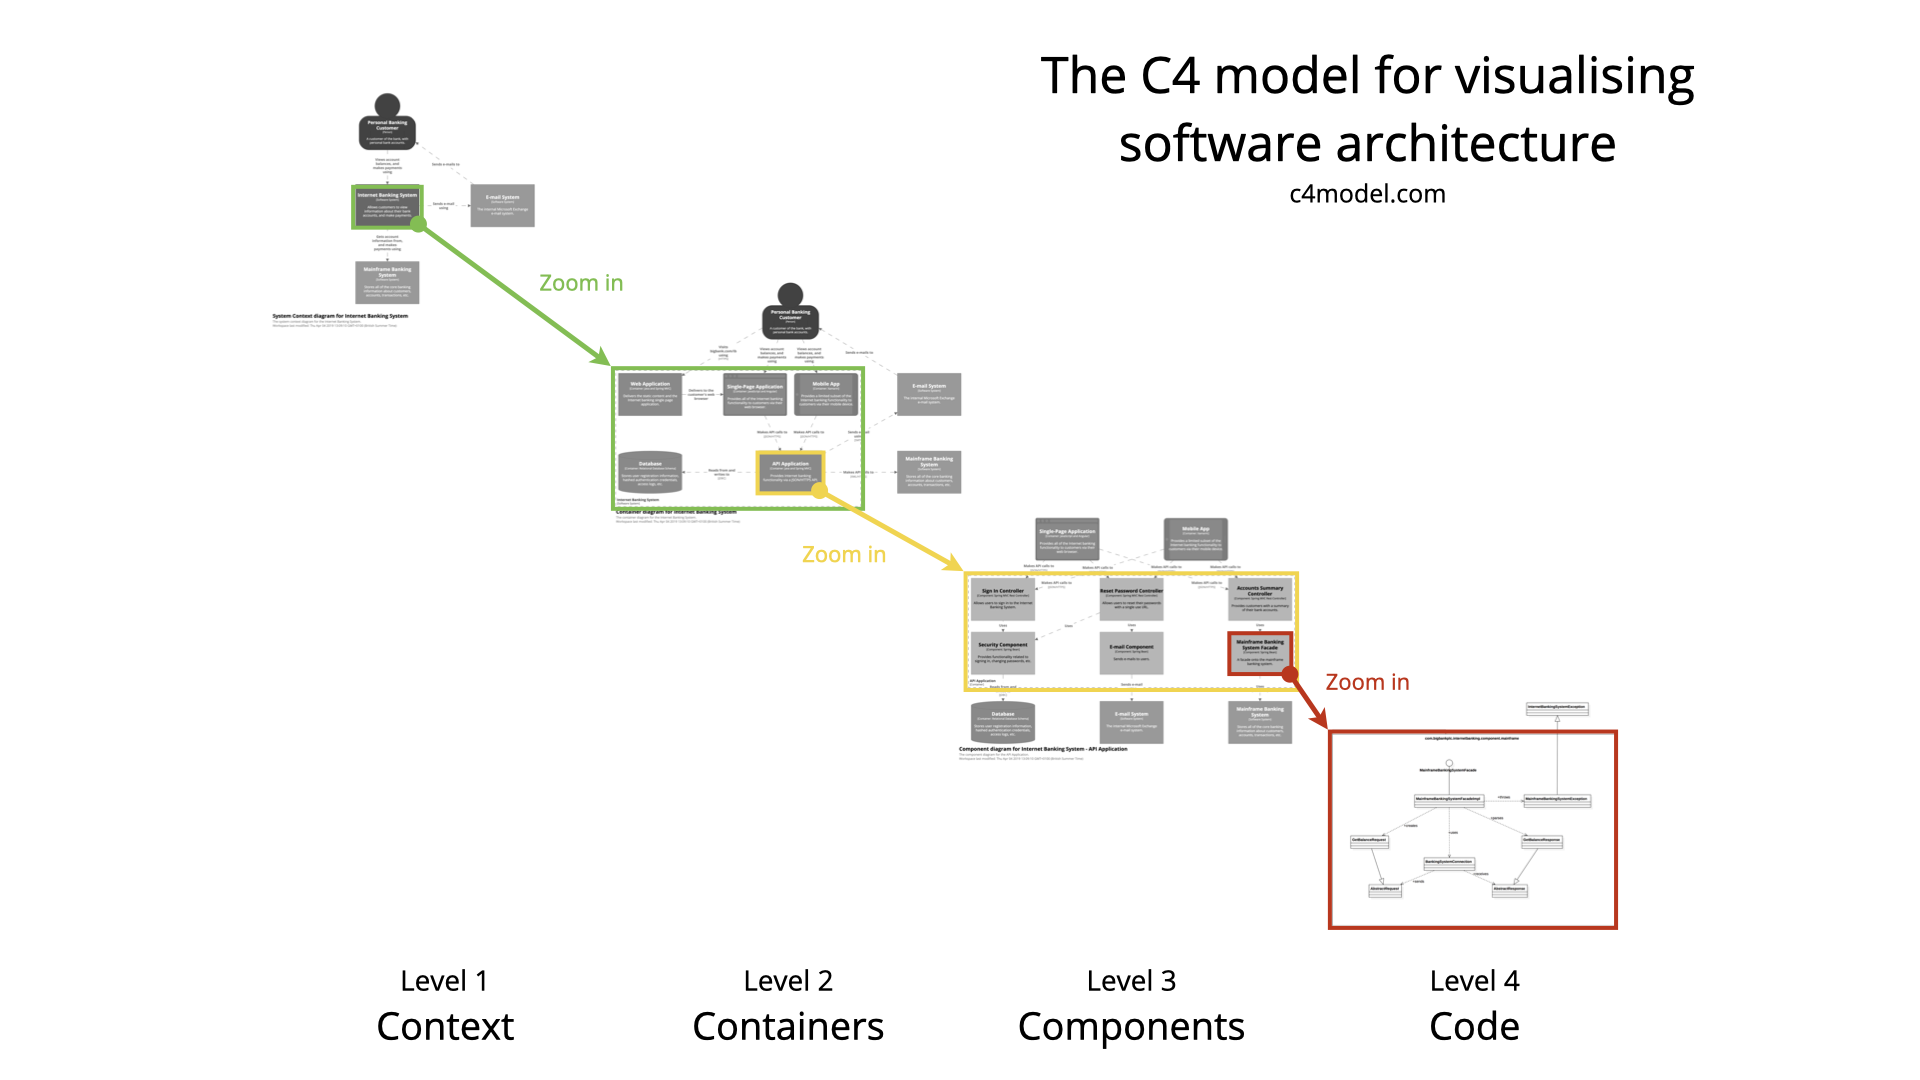
\includegraphics[width=\linewidth,keepaspectratio]{frontmatter/assets/diagrams/c4-overview.png}
    \caption{Modelo Arquitural C4}
    \label{fig:c4model}
\end{figure}

A granularidade do nível 4 revela-se excessiva e retira o foco aos diagramas que melhor ilustram a arquitetura do sistema, portanto, nao será abordado neste relatório.

\subsection{Modelo de Vistas 4+1}
\label{subsec:model4plus1}

Segundo \cite{Kruchten1995}, o modelo arquitetural "4+1" descreve a arquitetura de um sistema de \textit{software} a partir de cinco perspetivas complementares, cada uma focada em diferentes preocupações e públicos-alvo:

\begin{itemize}
\item \textbf{Vista Lógica} — Foca-se na funcionalidade do sistema, pois representa a estrutura dos principais componentes do domínio.

\item \textbf{Vista de Processos} — Descreve os aspectos dinâmicos do sistema, como a comunicação entre processos concorrentes e a forma como as tarefas são sincronizadas e distribuídas.

\item \textbf{Vista Física} — Mapeia os componentes de \textit{software} para os recursos de \textit{hardware} e ilustra como o sistema está distribuídoo.

\item \textbf{Vista de Implementação/Desenvolvimento} — Mostra a estrutura estática do código, organização em módulos/pacotes e o ambiente de desenvolvimento.

\item \textbf{Vista de Cenários} — Representa os principais casos de uso ou fluxos de interação do sistema.
\end{itemize}

\begin{figure}[H]
    \centering
    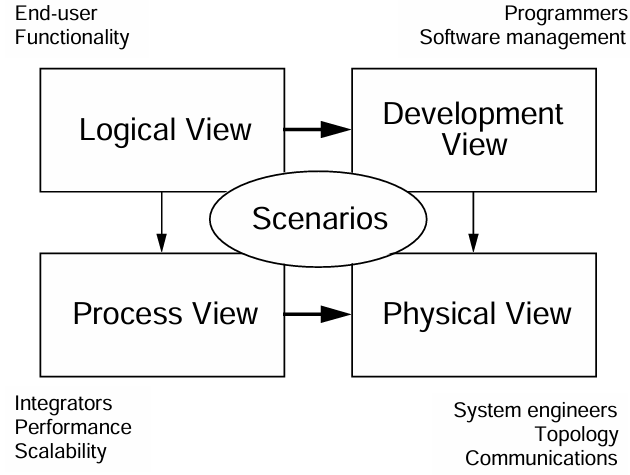
\includegraphics[width=3.5in,keepaspectratio]{frontmatter/assets/diagrams/4+1views.png}
    \caption{Modelo de Vistas 4+1}
    \label{fig:41viewmodel}
\end{figure}


\subsection{Vista de Processos}
\label{subsec:process_view}

Vários casos de uso têm fluxos muito semelhantes, alterando apenas o negócio em questão, como demonstrado no diagrama de vista de processo de nível 1, Figura \ref{fig:UC12345-lvl1} na secção \ref{sec:DP}.

De igual forma, os respetivos diagramas de nível 2 também partilham uma estrutura comum, diferenciando-se apenas na lógica de negócio subjacente. Esta semelhança é evidenciada na Figura \ref{fig:UC12345-lvl2}, que exemplifica uma dessas variações mantendo a arquitetura processual de base.

\begin{figure}[H]
\centering
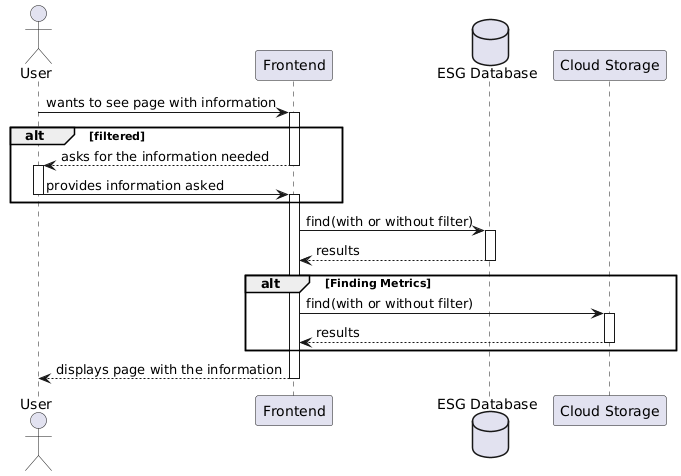
\includegraphics[width=5in]{frontmatter/assets/diagrams/Process Views/UC12345-lvl2.png}
\caption{Vista de processos dos casos de uso de consulta/visualização e filtragem (Nível 2)}
\label{fig:UC12345-lvl2}
\end{figure}

É ao nível 3 que se tornam evidentes as diferenças nos fluxos de interação, consoante os requisitos de cada funcionalidade. Como ilustrado na Figura \ref{fig:UC134-lvl3}, os casos de uso UC-01, UC-03 e UC-04 envolvem apenas o acesso à base de dados. Já o caso UC-05 (Figura \ref{fig:UC5-lvl3}) inclui também comunicação com o serviço de armazenamento na nuvem. A UC-02 (Figura \ref{fig:UC2-lvl3}) distingue-se ainda por incluir uma etapa de filtragem adicional antes da obtenção dos dados.


\begin{figure}[H]
\centering
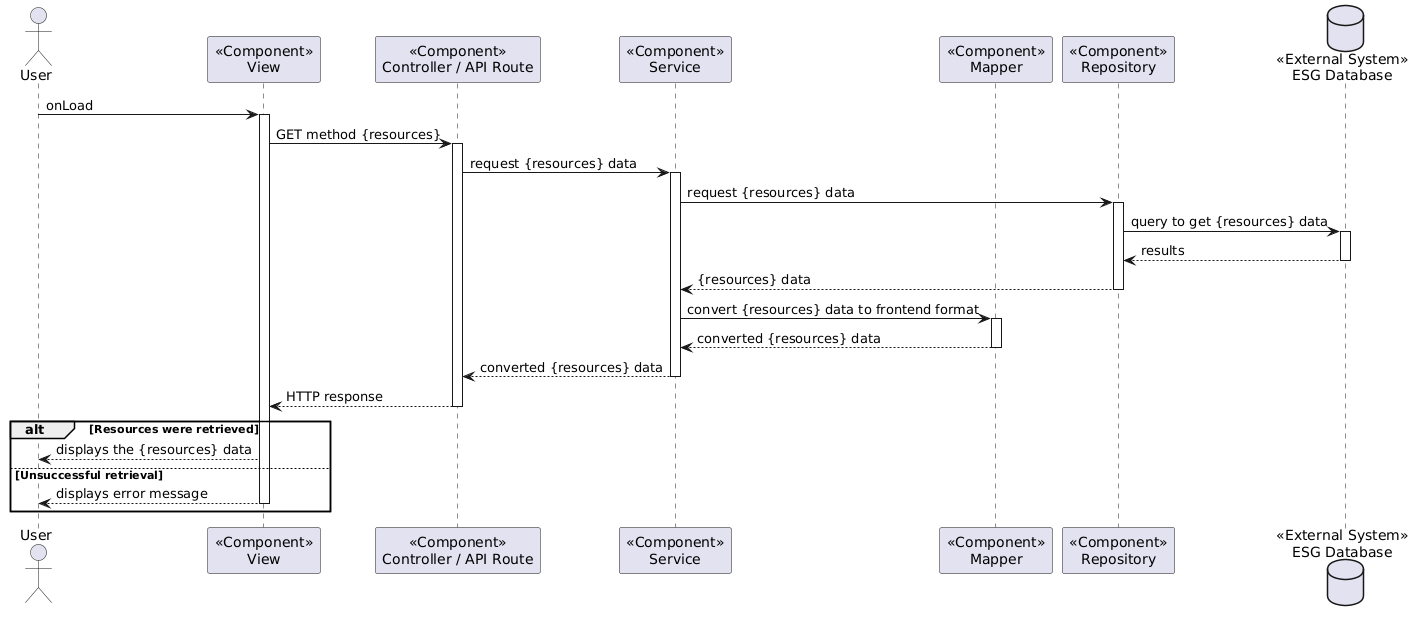
\includegraphics[width=\linewidth]{frontmatter/assets/diagrams/Process Views/LVL3/uc134-lvl3.png}
\caption{Vista de processos dos casos de uso de consulta (Nível 3)}
\label{fig:UC134-lvl3}
\end{figure}


\begin{figure}[H]
\centering
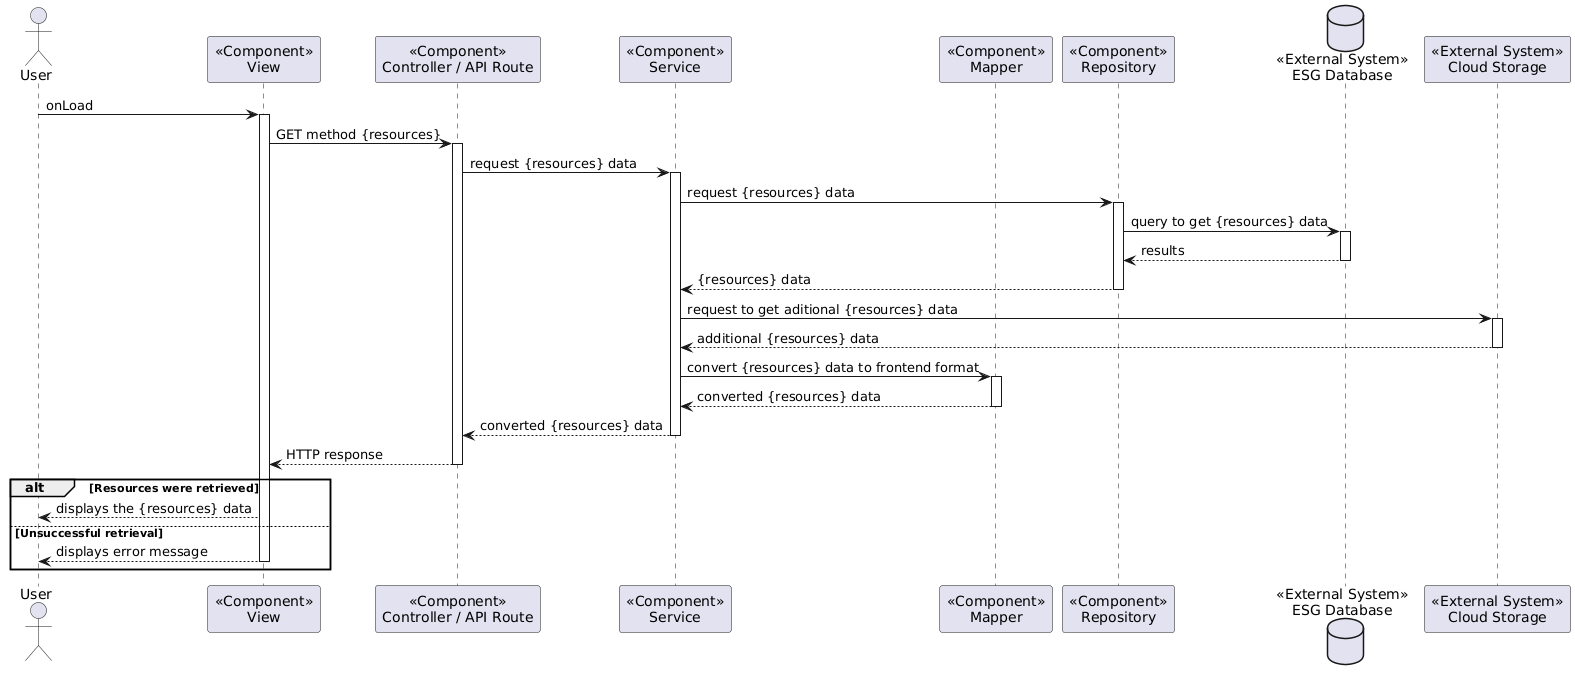
\includegraphics[width=\linewidth]{frontmatter/assets/diagrams/Process Views/LVL3/uc-05-lvl3.png}
\caption{Vista de processo do caso de uso de consulta com acesso ao armazenamento na nuvem (Nível 3)}
\label{fig:UC5-lvl3}
\end{figure}


\begin{figure}[H]
\centering
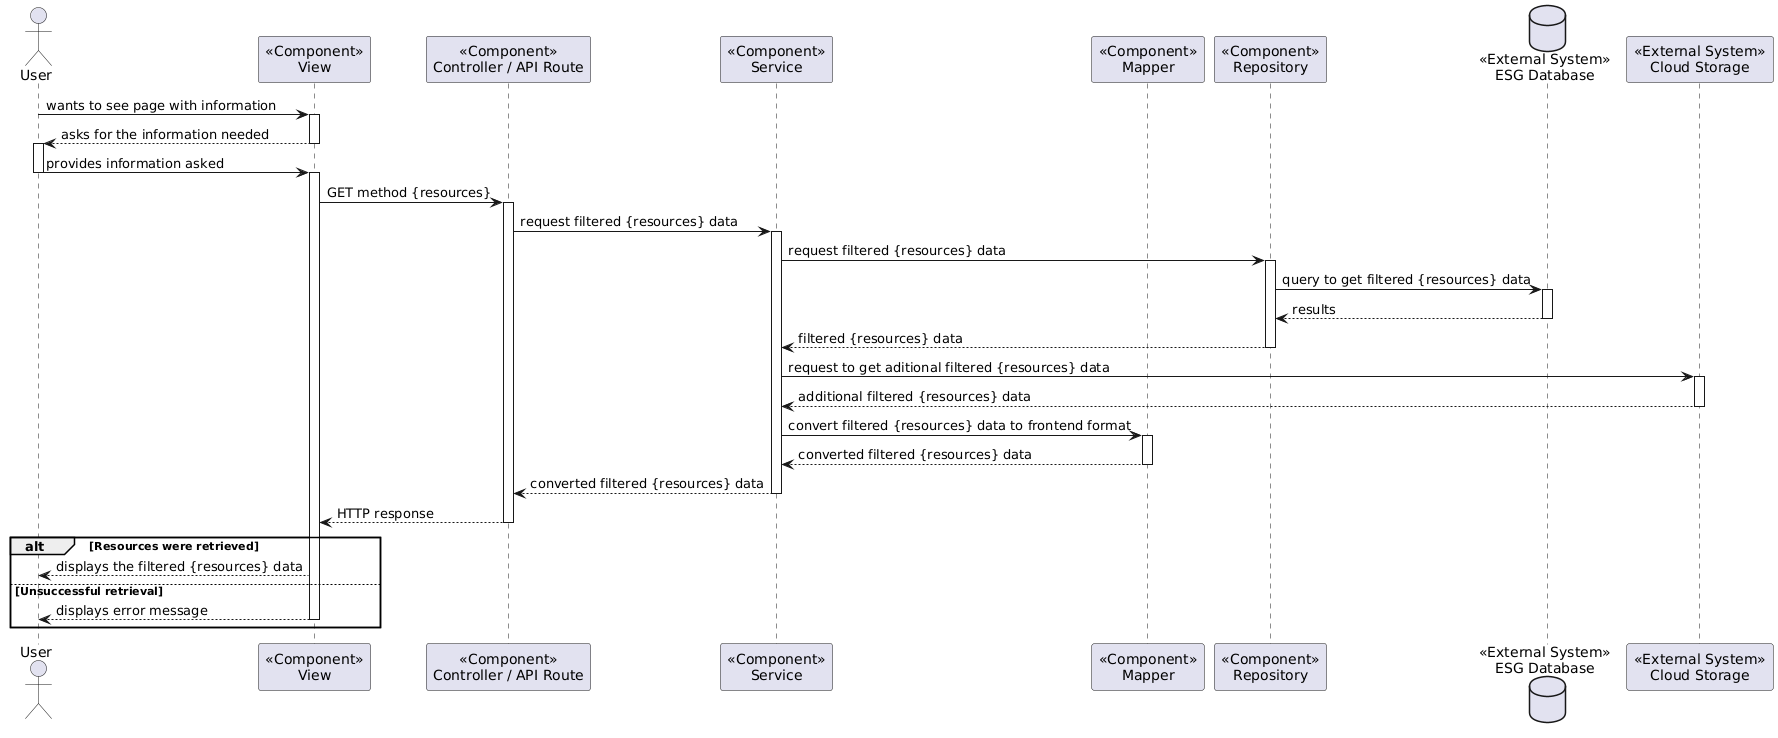
\includegraphics[width=\linewidth]{frontmatter/assets/diagrams/Process Views/LVL3/uc-02-lvl3.png}
\caption{Vista de processo do caso de uso de filtragem (Nível 3)}
\label{fig:UC2-lvl3}
\end{figure}

Da mesma forma, no nível 1, ambas os casos de uso UC-06 e UC-07 são bastante semelhantes, mudando apenas a lógica do negócio, como ilustrado na Figura \ref{fig:UC67-lvl1}.

\begin{figure}[H]
\centering
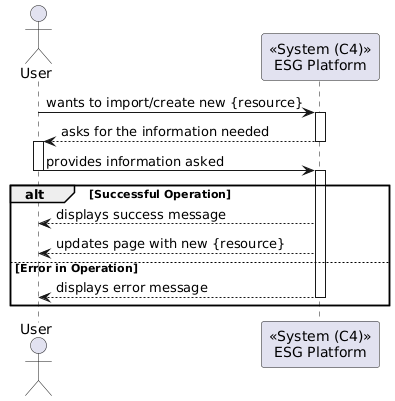
\includegraphics[width=3.5in]{frontmatter/assets/diagrams/Process Views/UC67-lvl1.png}
\caption{Vista de processo dos casos de uso de criação e importe (Nível 1)}
\label{fig:UC67-lvl1}
\end{figure}

A mesma tendência continua no nível seguinte, como é representado pela Figura \ref{fig:UC67-lvl2}.

\begin{figure}[H]
\centering
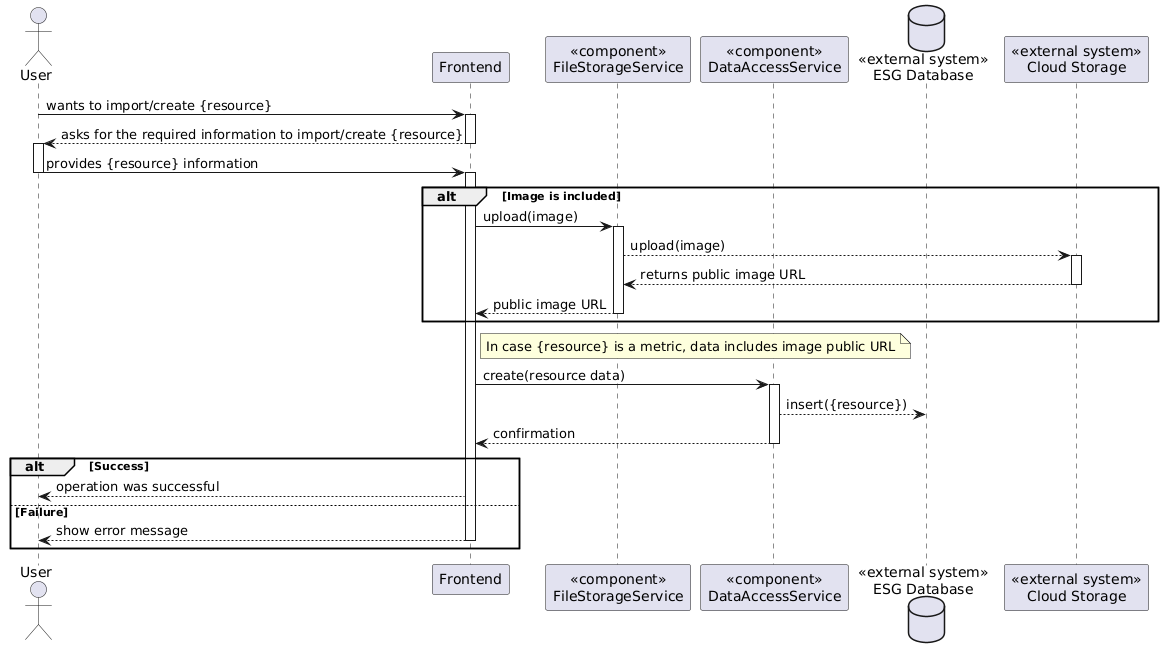
\includegraphics[width=\linewidth]{frontmatter/assets/diagrams/Process Views/UC67-lvl2.png}
\caption{Vista de processo dos casos de uso de criação e importe (Nível 2)}
\label{fig:UC67-lvl2}
\end{figure}

Novamente, a diferença entre estes dois casos de uso, UC-06 e UC-07, é realçada pelo diagrama de granularidade de nível 3, como se pode ver nas Figuras \ref{fig:UC6-lvl3} e \ref{fig:UC7-lvl3}, respetivamente.


\begin{figure}[H]
\centering
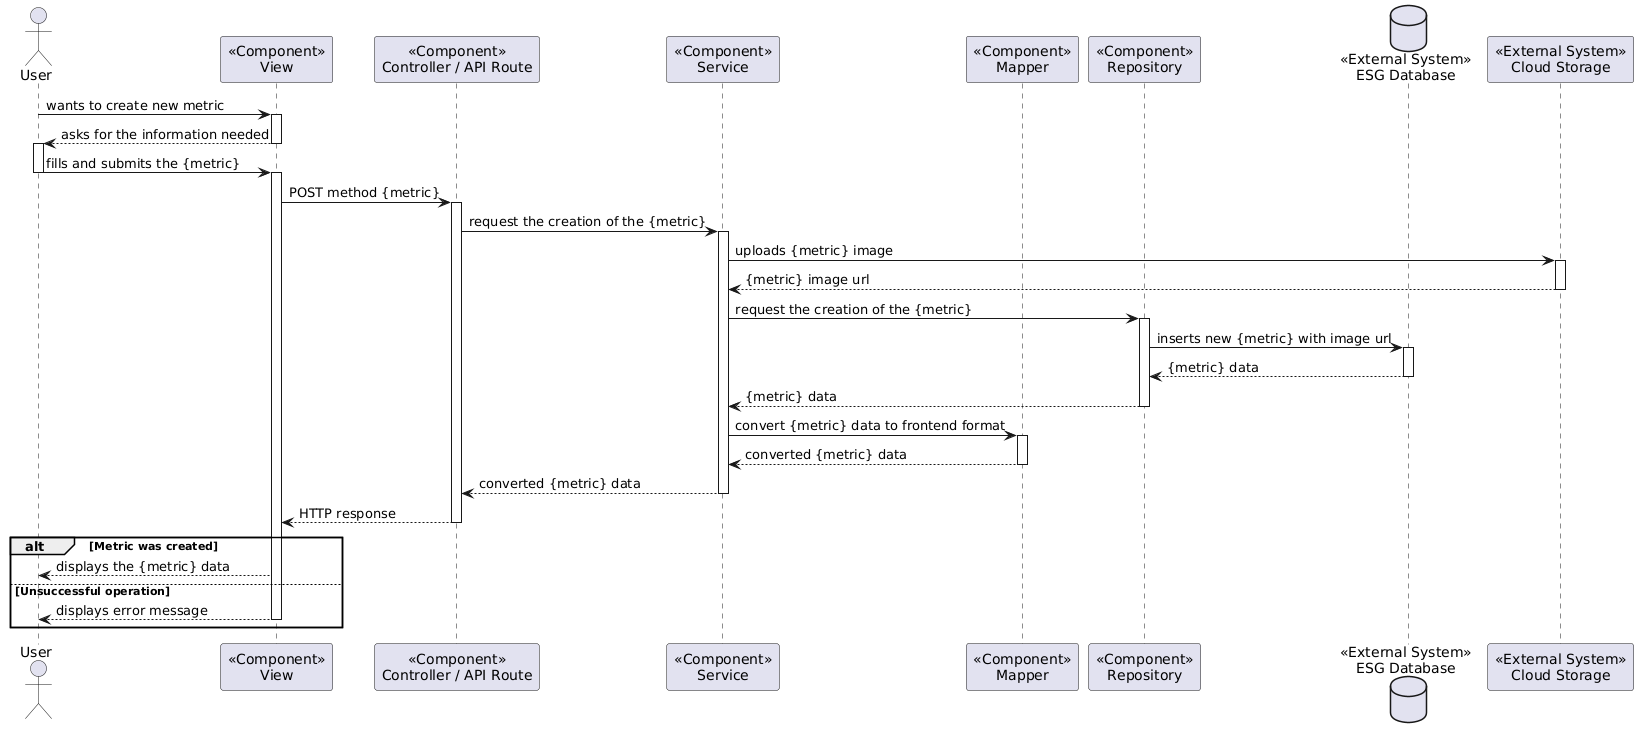
\includegraphics[width=\linewidth]{frontmatter/assets/diagrams/Process Views/LVL3/uc-06-lvl3.png}
\caption{Vista de processo do caso de uso de criação de métricas (Nível 3)}
\label{fig:UC6-lvl3}
\end{figure}

\begin{figure}[H]
\centering
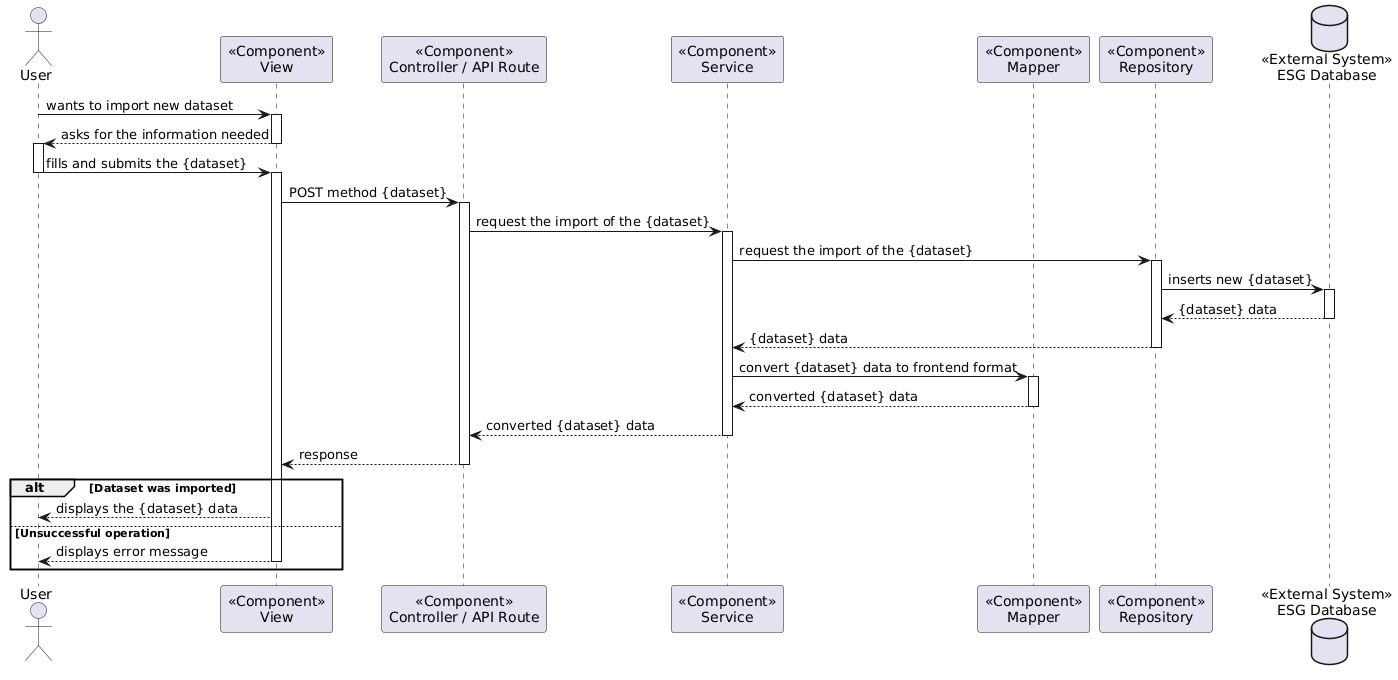
\includegraphics[width=\linewidth]{frontmatter/assets/diagrams/Process Views/LVL3/uc-07-lvl3.png}
\caption{Vista de processo dos casos de uso de importe de dados (Nível 3)}
\label{fig:UC7-lvl3}
\end{figure}


\subsection{Vista de Cenários}

A vista de cenários, ilustrada pela Figura \ref{fig:scenario_view}, compila os caso de usos mais gerais, no fundo, sendo uma abstração dos requisitos mais importantes, já explorados no capítulo anterior. Esta vista é vista como redundante, daí o "+1" na designação do modelo arquitetural (\cite{Kruchten1995}).

\begin{figure}[H]
    \centering
    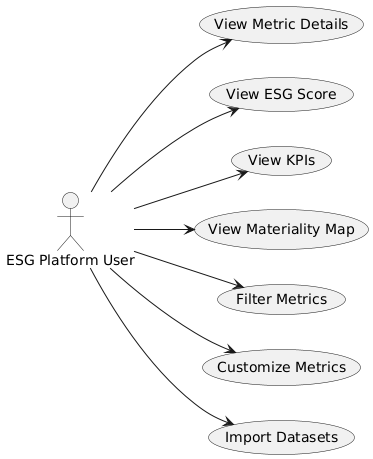
\includegraphics[height=4in,keepaspectratio]{frontmatter/assets/diagrams/Scenario View/Scenario_View.png}
    \caption{Vista de Cenários}
    \label{fig:scenario_view}
\end{figure}

\subsection{Vista Lógica}

Esta vista será abordada por vários diagramas correspondentes a sucessivos níveis de detalhe na representação logica do sistema, iniciando-se pelo nível 1, com a Figura \ref{fig:logical_view_lv1}, que permite entender o que o sistema disponibiliza, assim como que APIs consume.

\begin{figure}[H]
    \centering
    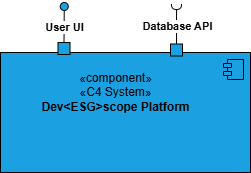
\includegraphics[width=2.5in,keepaspectratio]{frontmatter/assets/diagrams/Logical View/Logical View Lv1.drawio.png}
    \caption{Vista Lógica (Nível 1)}
    \label{fig:logical_view_lv1}
\end{figure}

A Figura \ref{fig:logical_view_lv2} apresenta o Nível 2, oferecendo uma visão mais detalhada do sistema. Este nível inclui o contentor \textit{Visualization}, responsável por disponibilizar a \textit{User UI}, através da qual os utilizadores interagem com a aplicação. Este contentor consome duas APIs, a \textit{Database API} e a \textit{Cloud Storage API}, que, respetivamente, comunicam com a base de dados e com o serviço de armazenamento na nuvem.

\begin{figure}[H]
    \centering
    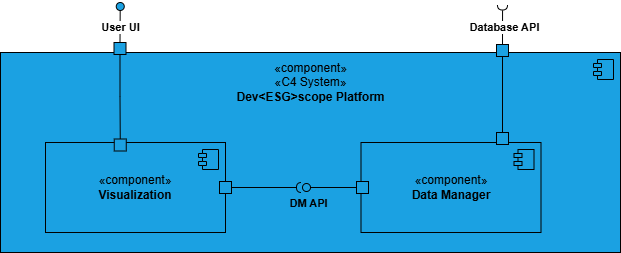
\includegraphics[width=4in,keepaspectratio]{frontmatter/assets/diagrams/Logical View/Logical View Lv2.drawio.png}
    \caption{Vista Lógica (Nível 2)}
    \label{fig:logical_view_lv2}
\end{figure}

Já o Nível 3 (Figura \ref{fig:logical_view_lv3}) representa os componentes que compõem os contentores do sistema, tornando mais claras as interações entre eles.

Observa-se que o contentor \textit{Visualization} consome duas APIs: uma disponibilizada pelo \textit{Database Provider} e outra pelo \textit{Cloud Storage Provider}.

O \textit{Cloud Storage Provider} contém um componente baseado no serviço Amazon S3, utilizado para armazenar ficheiros estáticos (como imagens) e gerar URLs de acesso público. Estes URLs são posteriormente armazenados na base de dados.

O \textit{Database Provider}, por sua vez, utiliza uma base de dados \textit{MySQL} hospedada na plataforma \textit{Railway}. A responsabilidade de persistir os dados, incluindo os URLs gerados, cabe ao contentor \textit{Visualization}, que interage diretamente com ambas as APIs.

\begin{landscape}
\begin{figure}[p]
    \centering
    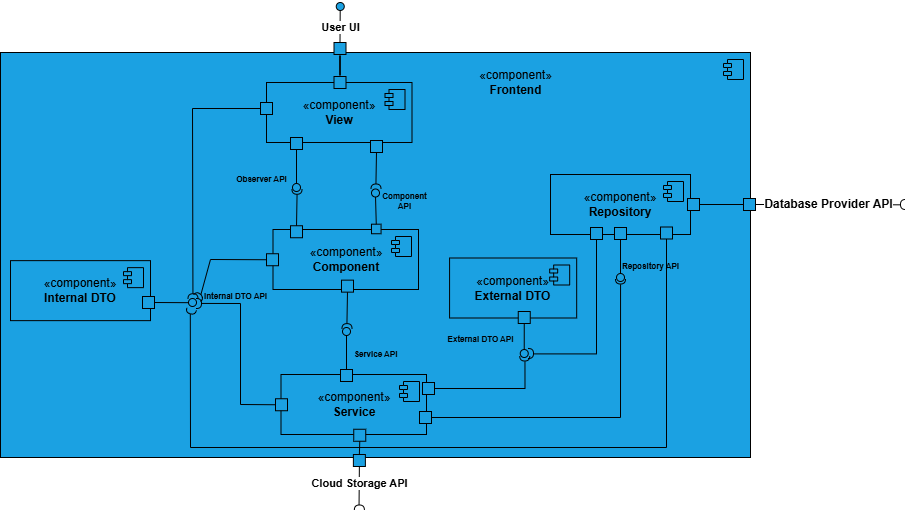
\includegraphics[width=\linewidth,keepaspectratio]{frontmatter/assets/diagrams/Logical View/Logical View Lv3.drawio.png}
    \caption{Vista Lógica (Nível 3)}
    \label{fig:logical_view_lv3}
\end{figure}
\end{landscape}

\subsection{Vista de Implementação}

Semelhante à subseção anterior, esta vista será detalhada em dois diagramas de diferentes granularidades, nível 2 e 3, representados, respetivamente, pelas Figuras \ref{fig:development_view_lv2} e \ref{fig:development_view_lv3}.

O nível 1 não consta neste relatório por se tratar de uma representação demasiado abstrata, que pouco acrescentaria ao entendimento do sistema em questão.

O nível 2 permite identificar os diferentes módulos que compõem a aplicação, bem como as interações entre eles. A \textit{Plataforma ESG} é constituída por um módulo de \textit{Frontend}, responsável pela interface visual através da qual os utilizadores interagem, e por dois módulos externos: o \textit{Cloud Storage Provider}, que armazena ficheiros estáticos (como imagens), e o \textit{Database Provider}, onde residem os dados que serão apresentados no \textit{Frontend}.

\begin{figure}[H]
    \centering
    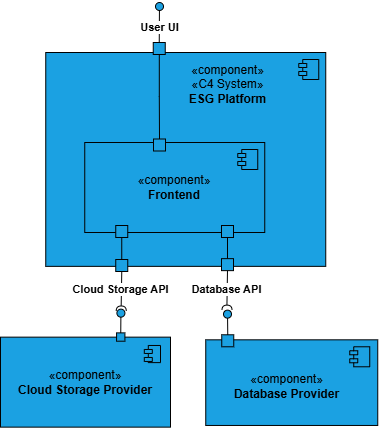
\includegraphics[width=3.5in,keepaspectratio]{frontmatter/assets/diagrams/Development View/Implementation View Lv2.drawio.png}
    \caption{Vista de Implementação Nível 2}
    \label{fig:development_view_lv2}
\end{figure}

Já o nível 3, de granularidade mais fina, elabora conteúdo do módulo \textit{Frontend}, dando um maior insight não só na sua constituição mas também nas diferentes interações entre os seus elementos 

A aplicação Plataforma ESG é constituida por uma React SPA para o \textit{Frontend}, construída para suportar a geração atual de browsers para desktop.

Todas as ações realizadas pelos utilizadores têm origem no \textit{Frontend}, que comunica com o \textit{Database Provider} para obter ou inserir os dados necessários. No caso específico da criação de uma nova métrica, o \textit{Frontend} interage adicionalmente com o \textit{Cloud Storage Provider}, onde ocorre o \textit{upload} da imagem representativa da respetiva métrica.

\begin{figure}[H]
    \centering
    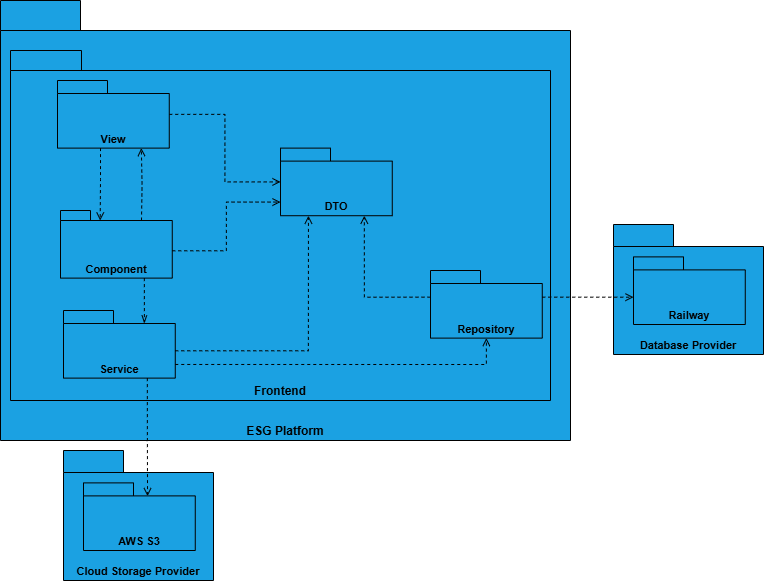
\includegraphics[width=\linewidth,keepaspectratio]{frontmatter/assets/diagrams/Development View/Implementation Lv3.drawio.png}
    \caption{Vista de Implementação Nível 3}
    \label{fig:development_view_lv3}
\end{figure}
    
\subsection{Vista Física}

A \textbf{vista física} tem como objetivo mapear o \textit{software} para o \textit{hardware}, com ênfase nos \textbf{requisitos não funcionais} do sistema, como disponibilidade,confiabilidade (tolerância a falhas), desempenho e escalabilidade (\cite{Kruchten1995}). A Figura~\ref{fig:physical_view_lv2} apresenta o diagrama de nível 2 da vista física da solução desenvolvida.

Os \textbf{Load Balancers} são responsáveis por distribuir o tráfego de forma dinâmica entre os servidores que compõem as camadas de \textit{Visualization} (\textit{frontend}) e \textit{Data Management} (\textit{backend} com base de dados). Estes atuam como intermediários entre os utilizadores e os servidores, assegurando uma \textbf{distribuição equilibrada da carga}, especialmente durante períodos de maior tráfego. Com isso, aumentam a disponibilidade e a resiliência do sistema: caso um servidor falhe, o tráfego é automaticamente redirecionado para outro servidor ativo (tolerância a falhas). Esta abordagem contribui ainda para a redução da latência e para evitar respostas inconsistentes da aplicação (\Cite{F52025}).

As comunicações entre os vários componentes são realizadas através de protocolo HTTP ou HTTPS.

\begin{figure}[H]
    \centering
    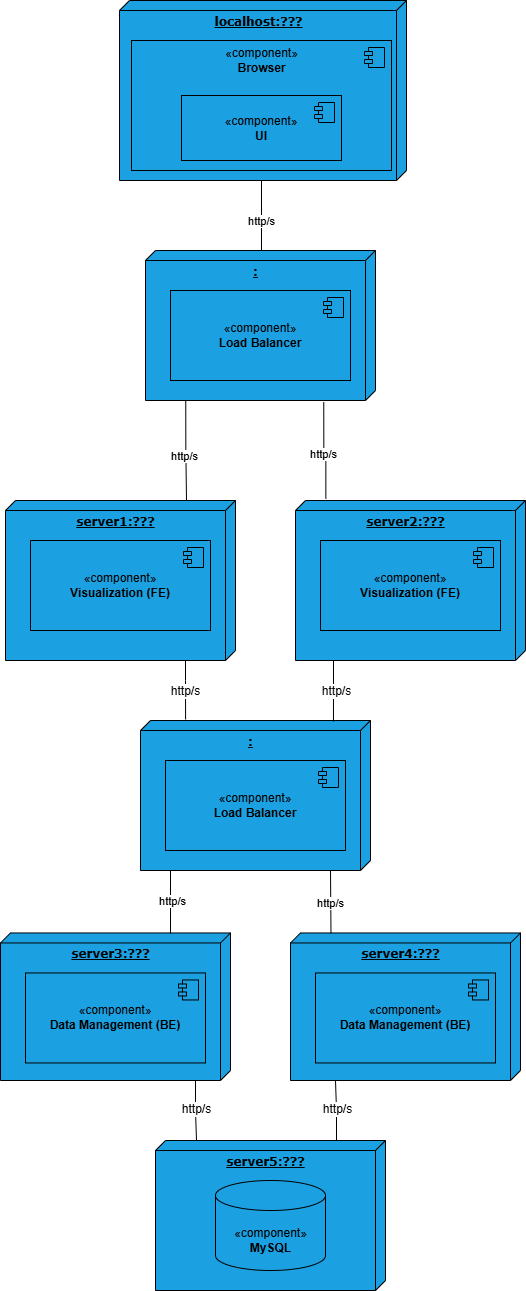
\includegraphics[height=8in,keepaspectratio]{frontmatter/assets/diagrams/Physical View/physical_view_lv2.drawio.png}
    \caption{Diagrama de nível 2 da vista física da solução}
    \label{fig:physical_view_lv2}
\end{figure}

\section{Alternativa Arquitetural: DDD com \textit{Clean Architecture}}
\label{sec:SolAlt}

Uma alternativa à arquitetura escolhida para estruturar o sistema em questão, baseada no modelo C4/4+1, seria a adoção de uma abordagem baseada em \textit{Domain-Driven Design} (DDD) combinada com os princípios da \textit{Clean Architecture}. Esta forma permite igualmente estruturar a aplicação de forma modular e escalável, de modo a respeitar os limites naturais do domínio e manter a flexibilidade para futuras expansões.

Nesta solução alternativa, o sistema é dividido em módulos de domínio independentes, cada um a representar um conceito central da aplicação ESG: \textit{Dataset} (gestão de conjuntos de dados e unidades de medida), \textit{Metric} (definição e cálculo de métricas ESG, associadas a datasets e subáreas), \textit{Objective} (objetivos definidos com base em métricas e metas temporais), \textit{Pillar} e \textit{Subarea} (classificação temática e estrutural das métricas).

Cada domínio é responsável pelas suas entidades, regras de negócio e casos de uso, encapsulados em serviços de aplicação que orquestram a lógica. A comunicação com o exterior é feita através de interfaces (\textit{ports}), e a infraestrutura (como base de dados ou armazenamento na nuvem) implementa os adaptadores que servem essas mesmas interfaces.

A estrutura segue o modelo de anéis concêntricos proposto pela \textit{Clean Architecture}, onde o núcleo do sistema (as entidades de domínio) está isolado das dependências externas. A camada de aplicação contém os casos de uso que coordenam o fluxo de dados entre o domínio e o mundo exterior. À volta desta, encontram-se os adaptadores (como APIs ou repositórios) e, finalmente, a camada mais externa é composta por \textit{frameworks} e bibliotecas específicas (como Prisma ou Next.js).

Esta organização proporciona vários benefícios: isolamento claro de responsabilidades, evitação de acoplamento excessivo, maior facilidade de testes, e independência das tecnologias utilizadas, o que contribui para uma maior manutenibilidade e qualidade do código.

Desta forma, a aplicação mantém-se coesa, flexível e preparada para crescer de forma sustentável.